\documentclass[10pt, journal]{IEEEtran}
\usepackage{cite}
\usepackage{url}
\usepackage{graphicx}


\author{\IEEEauthorblockN{Remco Aarts}, 
 \IEEEauthorblockN{Jeroen van den Akker}, 
 \IEEEauthorblockN{Robert Delmaar}, 
 \IEEEauthorblockN{Bas Janssen},
 \IEEEauthorblockN{Addie Perenboom},
 \IEEEauthorblockN{Dimitri Waard}
 \IEEEauthorblockA{\\Minor Adaptive Robotics,
Fontys University of Applied Sciences\\
Eindhoven\\
Email: smh.janssen@student.fontys.nl}}

%\author{Remco Aarts, Jeroen van den Akker, Robert Delmaar, Bas Janssen, Addie Perenboom, Dimitri Waard}

\title{Decentralized multi-robot logistics}

\begin{document}
\maketitle

\begin{abstract}
This paper describes the design and implementation of a decentralized multi-robot logistics system. Both the hardware design and the software design and implementation are expanded upon below.
\end{abstract}
\begin{IEEEkeywords}

\end{IEEEkeywords}

\section{Introduction}
The decentralized multi-robot logistics project is one of the main projects of the Adaptive Robotics Minor at Fontys Hogeschool Engineering, in the 2016-2017 academic year. The goal of this project is to develop a system, both hardware and software, that is capable of transporting products between a warehouse and production locations in an Industry 4.0 setting. The system can be a replacement for a traditional conveyor belt, or can be used as a flexible addition to an existing conveyor system.
During this project the software making the decisions on the robots has been developed, built on top of the Robot Operating System\cite{ROS}. This software is designed to receive commands from one or more workstations, and have the robots decide which robot should execute a command. The robots have the ability to request help from one another if more products have to be transported than a single robot can carry, or it is beneficial to transfer one or more products between two robots to get the products to their destination faster.

\section{Hardware}
The turtlebots must transport carriages from one point in a warehouse/factory to another. In addition to this it was decided that the turtlebots have to be able to transfer carriages from one bot to another. A morphological chart was used to create multiple solutions for this task. The solutions that were most promising and realistic were worked out in detail. Initially the turtlebots were meant to have multiple specializations. These versions were also in the morphological chart, out of which two were chosen, but in the end, it was financially and time-wise not feasible to implement both specializations. Therefore only one concept was realized.
\subsection{Stackup}
The position of the camera was moved to the front of the turtlebot, beneath the disk the laptop is placed on top of. The system that holds the carriages and is capable of transferring them is mounted on top of the disk above the laptop.
%------------
\begin{figure}[htp]
\centering
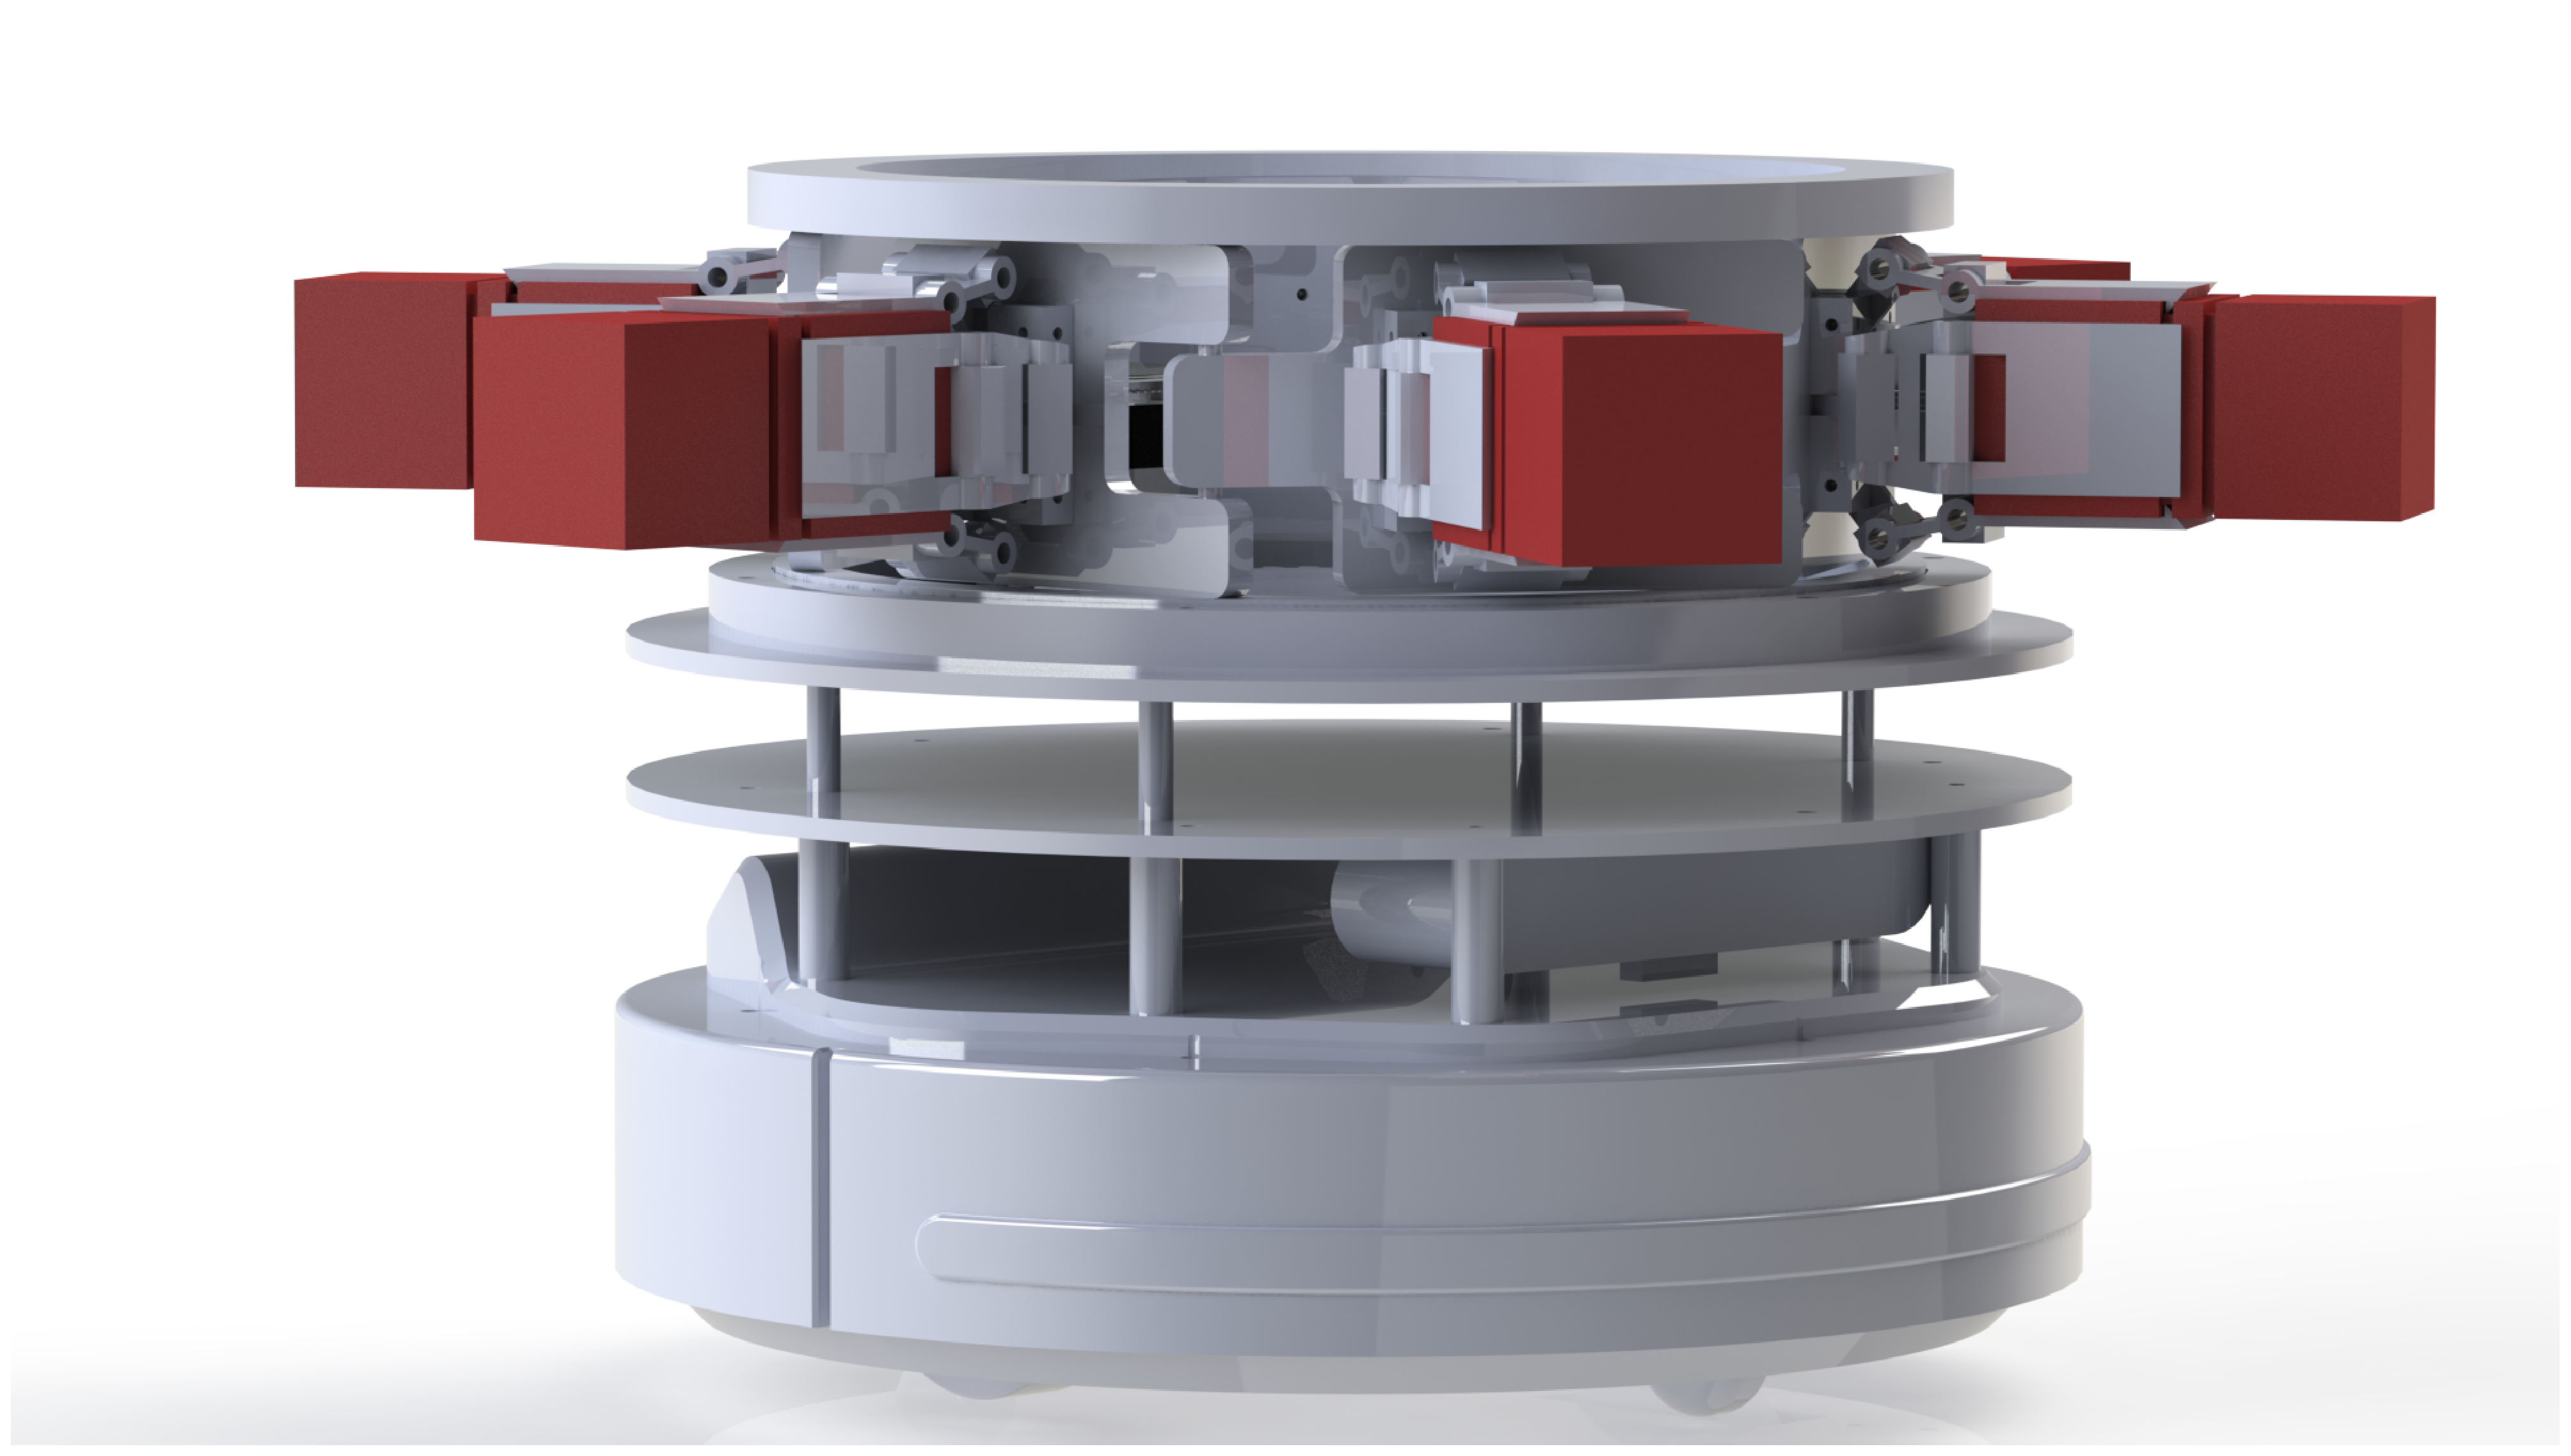
\includegraphics[width=\columnwidth]{turtle_design}
\caption{Mechanical Design}
\label{MechanicalDesign}
\end{figure}
%------------
%----------------
\begin{figure}[htp]
\centering
\includegraphics[width=\columnwidth]{gripper}
\caption{Gripper}
\label{Gripper}
\end{figure}
%--------------
Six grippers are mounted on the turtlebot, each can carry a single carriage. To align the carriages for transfer the grippers can revolve around the turtlebot. For this purpose, the grippers and a stepper motor are mounted on top of a Lazy Suzan bearing. A smaller gear on the motor and a large gear on the plate make it possible for the bearing to revolve. A reed contact and a magnet are used to keep track of the position of the grippers instead of an encoder. A slip ring is used to keep the electrical cables from entangling or breaking loose because of the movement. This design is displayed in figure \ref{MechanicalDesign}.

\subsection{Gripper}
When a carriage is pushed into the gripper a plate with an axle attached to it will be pushed back. Pushing the plate back will cause the fingers to grip the carriage. The gripper will be mechanically locked by the axle, to be released by a servo. When released a spring pushes the plate back, causing the gripper to open. The carriages will be pushed into the gripper by driving the turtlebot against it. To get the alignment right the gripper is revolved around the turtlebot first.

The carriages are a standard size of 50 by 50 by 100 millimeters and are intended to carry small parts such as bolts. A photograph of the gripper is shown in figure \ref{Gripper}.

\section{Software}

\subsection{Distance calulation}
The robots make independent decisions, whether to accept a request, based on their available inventory space, and the distance between the robot and the goal. The length $s$ of the planned path is calculated using equation \ref{eq_pathlength}, where $x$ and $y$ represent the x and y coordinate of a point in the path. This means that for each point $i$ in the path, the distance to the next point is calculated. The length is the sum of these distances.
\begin{equation}
\label{eq_pathlength}
s= \sum\limits_{i=0}^j \sqrt{(y_i - y_{i+1})^2 + (x_i - x_{i+1})^2}
\end{equation}

\subsection{Multimaster-fkie}
All robots in the group communicate with each other. As each robot is its own ROS master, the normal way of using multiple machines \cite{ROSMultipleMachines} in the ROS ecosystem is not viable. However, a package capable of communicating between multiple independent ROS masters has been developed, called multimaster-fkie \cite{Multimaster-fkie}. Using this package it is possible to synchronize one or more topics between one or more ROS masters. This project uses said functionality to synchronize the command and control topics for the robots between the robots and the workstations.

The multimaster package provides two nodes, namely master-discovery and master-sync. The master-discovery node uses a multicast address to find the other masters on the network, and this list of masters is passed to the master-sync node to synchronize the specified topics.
\subsection{Simulation}
To test the software during development a simulation in Gazebo\cite{Gazebo} has been configured\cite{MultipleRobots}. The simulation has been configured for four robots, because the computer systems available could not simulate more robots at the same time with reasonable performance. Four robots also allows for testing the collaborative operation and provides the capability to have multiple robots running multiple different commands.

Within Gazebo, the complete robots and the world are fully simulated. This means that the robots are subject to simulated physics, collisions are possible and the entire software stack for each robot is running. This means that for each robot a move\_base controller, a depthimage-to-laserscan, a pathplanner and the decision software is launched. To complete the simulation, a virtual world has been built for the robots to move around in. This world consists of eight one by one by one meter cubes that represent obstacles. The cubes are spaced throughout this virtual world.
%------------
\begin{figure}[htp]
\centering
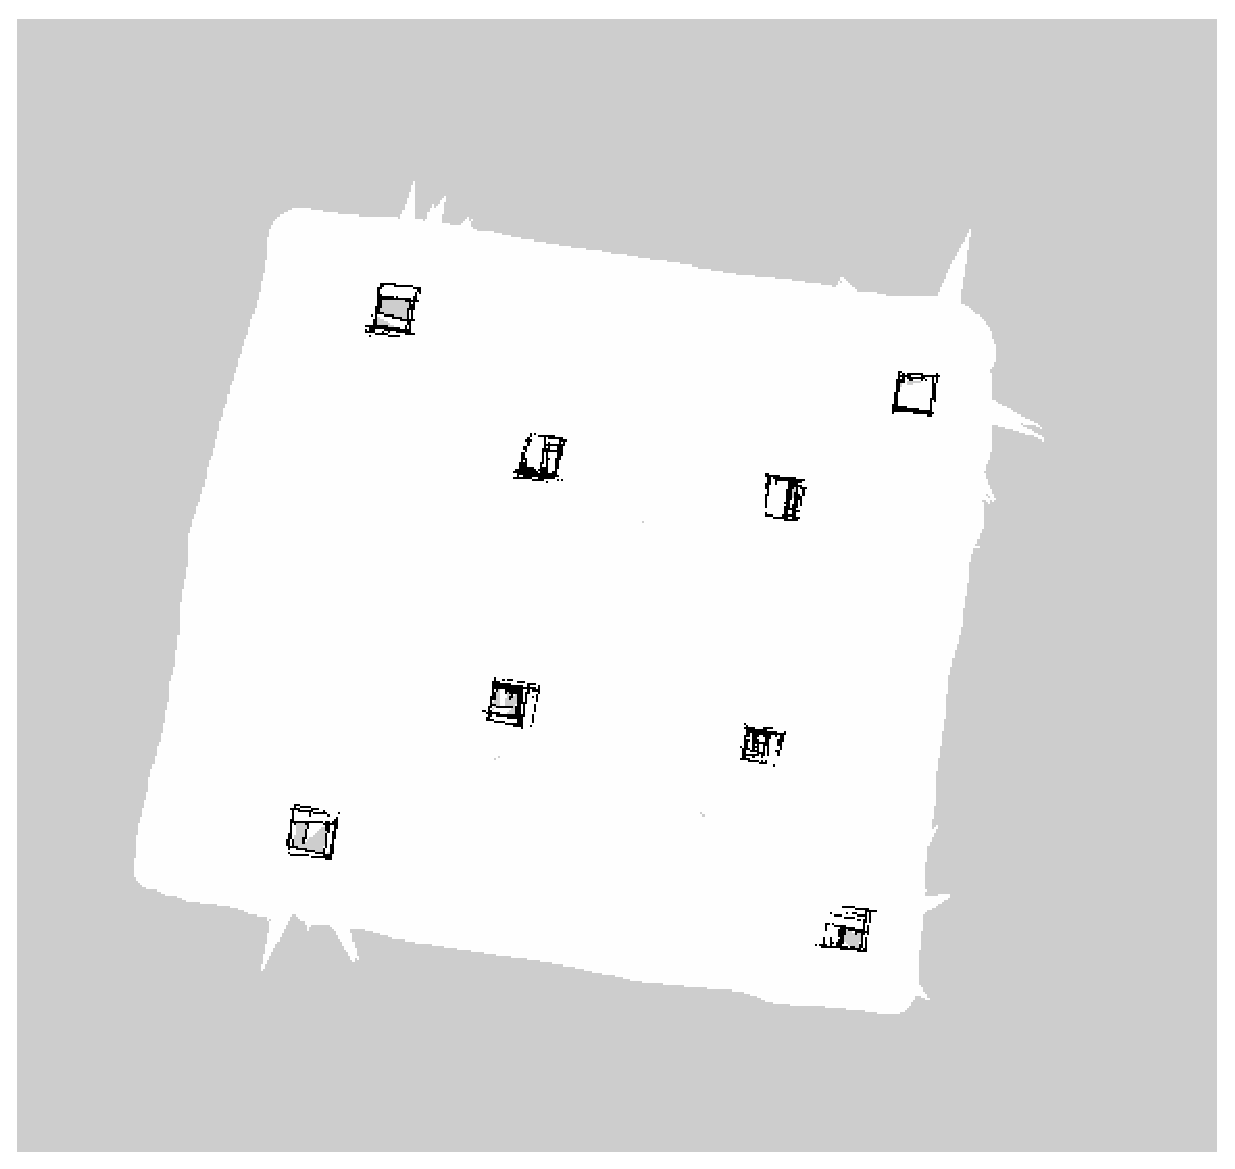
\includegraphics[width=\columnwidth]{gazebo_2}
\caption{Map of the simulated world, depicting the known area in white, the know obstacles in black and the unknown area in grey.}
\label{SimulatedWorldMap}
\end{figure}
%---------------
Figure \ref{SimulatedWorldMap} shows the map of this virtual world generated with gmapping SLAM package\cite{SLAMGmapping}, and edited to expand the known area, as mapping the entire simulated world would take to long using a turtlebot. By editing the image in GIMP\cite{GIMP}, no information is lost, as the obstacles stay in the same location. The white area represents the known area, grey represents unknown and the black markings are the detected obstacles.
\subsection{Software scales to more robots}
The software has been designed to scale to an unlimited number of robots. The only limitation is that the systems running the robots have enough RAM to store all the information for the robots.
\section{Results}
During testing, it was determined that the turtlebots are not suitable for this application. The odometry of the turtlebots is lacking, and very error prone. The Orbbec Astra RGBD camera placed on the turtlebot is not very suitable as a simulated laserscanner, as the resolution and update rate are too low to provide detailed information. It is therefore recommended to replace the turtlebots with a more suitable robot platform if this system is to be taken further than the proof of concept phase.

\bibliographystyle{IEEEtran}
\bibliography{paper_multirobot_logistics}
\end{document}